% !TEX program = xelatex
\documentclass[11pt,aspectratio=169]{beamer}

\makeatletter
\def\@makefnmark{}
\makeatletter

\setbeamersize{text margin left=5mm,text margin right=5mm} 

\usepackage{amsthm,amsmath,amssymb,braket,fontspec}
\usepackage[absolute,overlay]{textpos}

\usetheme[numbering=none,nofirafonts]{focus}

\setbeamercolor{footnote}{fg=blue}
\setbeamerfont{footnote}{size=\small}
\setbeamertemplate{bibliography item}[triangle]

\setmainfont{Fira Sans}
\setsansfont{Fira Sans}
\setbeamerfont{title}{size=\LARGE, shape=\scshape}
\setbeamerfont{author}{size=\large, shape=\scshape}
\setbeamerfont{institute}{size=\normalsize, shape=\scshape}
\setbeamerfont{date}{size=\normalsize, shape=\scshape}
\setbeamerfont{frametitle}{size=\large, shape=\scshape}

\usepackage[backend=bibtex,url=false,doi=false,maxcitenames=1, style=authoryear]{biblatex}
\bibliography{bib}
\AtBeginBibliography{\scriptsize}

\newcommand{\focus}[1]{\textcolor{red}{#1}}

\definecolor{red}{HTML}{CC0000}
\setbeamertemplate{bibliography item}[triangle]

\AtBeginSection[]{
\begin{frame}
  \vfill
  \centering
  \begin{beamercolorbox}[sep=20pt,rounded=true,center]{frametitle}
    \usebeamerfont{title}\insertsectionhead\par%
  \end{beamercolorbox}
  \vfill
\end{frame}
}
\title{
{Hierarchical structure and topological content of entanglement of free fermions}
}
\date{\today}
\author{Abhirup Mukherjee, Siddhartha Patra, Siddhartha Lal}
\institute{Department of Physical Sciences, IISER Kolkata, Mohanpur}
\date{\today}

\begin{document}

\centering

\begin{frame}
\maketitle
\begin{textblock*}{0.4\textwidth}(5.5cm, 6.5cm)
	\centering
	\vspace*{\fill}

	\includegraphics[width=0.35\textwidth]{figures/epqm_logo_mod.jpeg}
	\hspace*{\fill}
	\includegraphics[width=0.35\textwidth]{figures/dps_logo.jpeg}

	\vspace*{\fill}
\end{textblock*}
\end{frame}

\section{Introduction}

\begin{frame}{The system}

{Massless Dirac fermions on a 2-torus}
\[\mathcal{L} = i\int \mathrm{d}x~\mathrm{d}y~\overline\psi\gamma_\mu\partial_\mu \psi\]
{In presence of an Aharonov-Bohm flux}
\[\mathcal{L} = \int \mathrm{d}x~\mathrm{d}y~\overline\psi \left(i\gamma_\mu + eA_\mu\right)\partial_\mu \psi\]
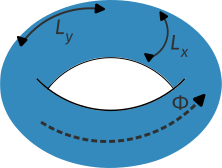
\includegraphics[width=0.4\textwidth]{figures/torus.pdf}
\hspace*{\fill}
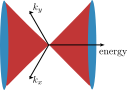
\includegraphics[width=0.42\textwidth]{figures/dirac.pdf}

\end{frame}

\begin{frame}[allowframebreaks]{Measures of entanglement}
	\begin{minipage}{0.6\textwidth}
		\(\rho = \ket{\Psi}\bra{\Psi}\longrightarrow\)\focus{density matrix}\\[10pt]
	\(\rho_A = \) partial trace over system A\\
	\(\longrightarrow\) \focus{reduced DM}\\[10pt]
	\(S(A) = -\text{Tr}\left[\rho_A \ln \rho_A\right] \)\\
	\(\longrightarrow\) \focus{entanglement entropy} of A\\[10pt]
	\end{minipage}
	\hspace*{\fill}
	\begin{minipage}{0.38\textwidth}
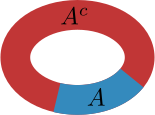
\includegraphics[width=\textwidth]{figures/subsystem-A.pdf}
\end{minipage}
\end{frame}


\begin{frame}[allowframebreaks]{References}
\printbibliography
\end{frame}

\end{document}
